\subsection{View}
The \emph{view}, which serves as the user interface, provides an interface for the user to interact with the application. The \emph{view} will be implemented as a graphical user interface (GUI) to enhance the user experience. 
It is responsible for displaying the pre-defined functionalities in \autoref{chap:model_design}, allowing users to easily navigate and use the features provided by the application. 
Several mock-ups have been designed using the UI design tool UIzard\footnote{UIzard is a UI design tool used for designing wireframes, mockups, and prototypes. Homepage: \url{https://uizard.io/}} to provide a clearer visualization of the layout of the user interface.

\subsubsection{HomeFragment}
The HomeFragment serves as the main screen of the application, providing an overview of the user's health and activity-related functionalities defined in \autoref{chap:hr_monitor_design}. This \emph{view} consists of various components, including real-time heart rate display and activity monitor.
The real-time heart rate display dynamically shows the user's live heart rate, allowing them to track their cardiovascular activity. Additionally, it features a dynamic graph that visualizes the user's heart rate history, which enables them to track their heart rate patterns over time.
The activity monitor informs the user's current activity intensity based on their current heart rate, which enables them to track their activity intensity and adjust their current activity intensity according to their needs. As mentioned in \autoref{chap:activity_intensity}, the intensity levels range from very light, light, moderate, hard, and very hard.

\begin{figure}[H]
    \centering
    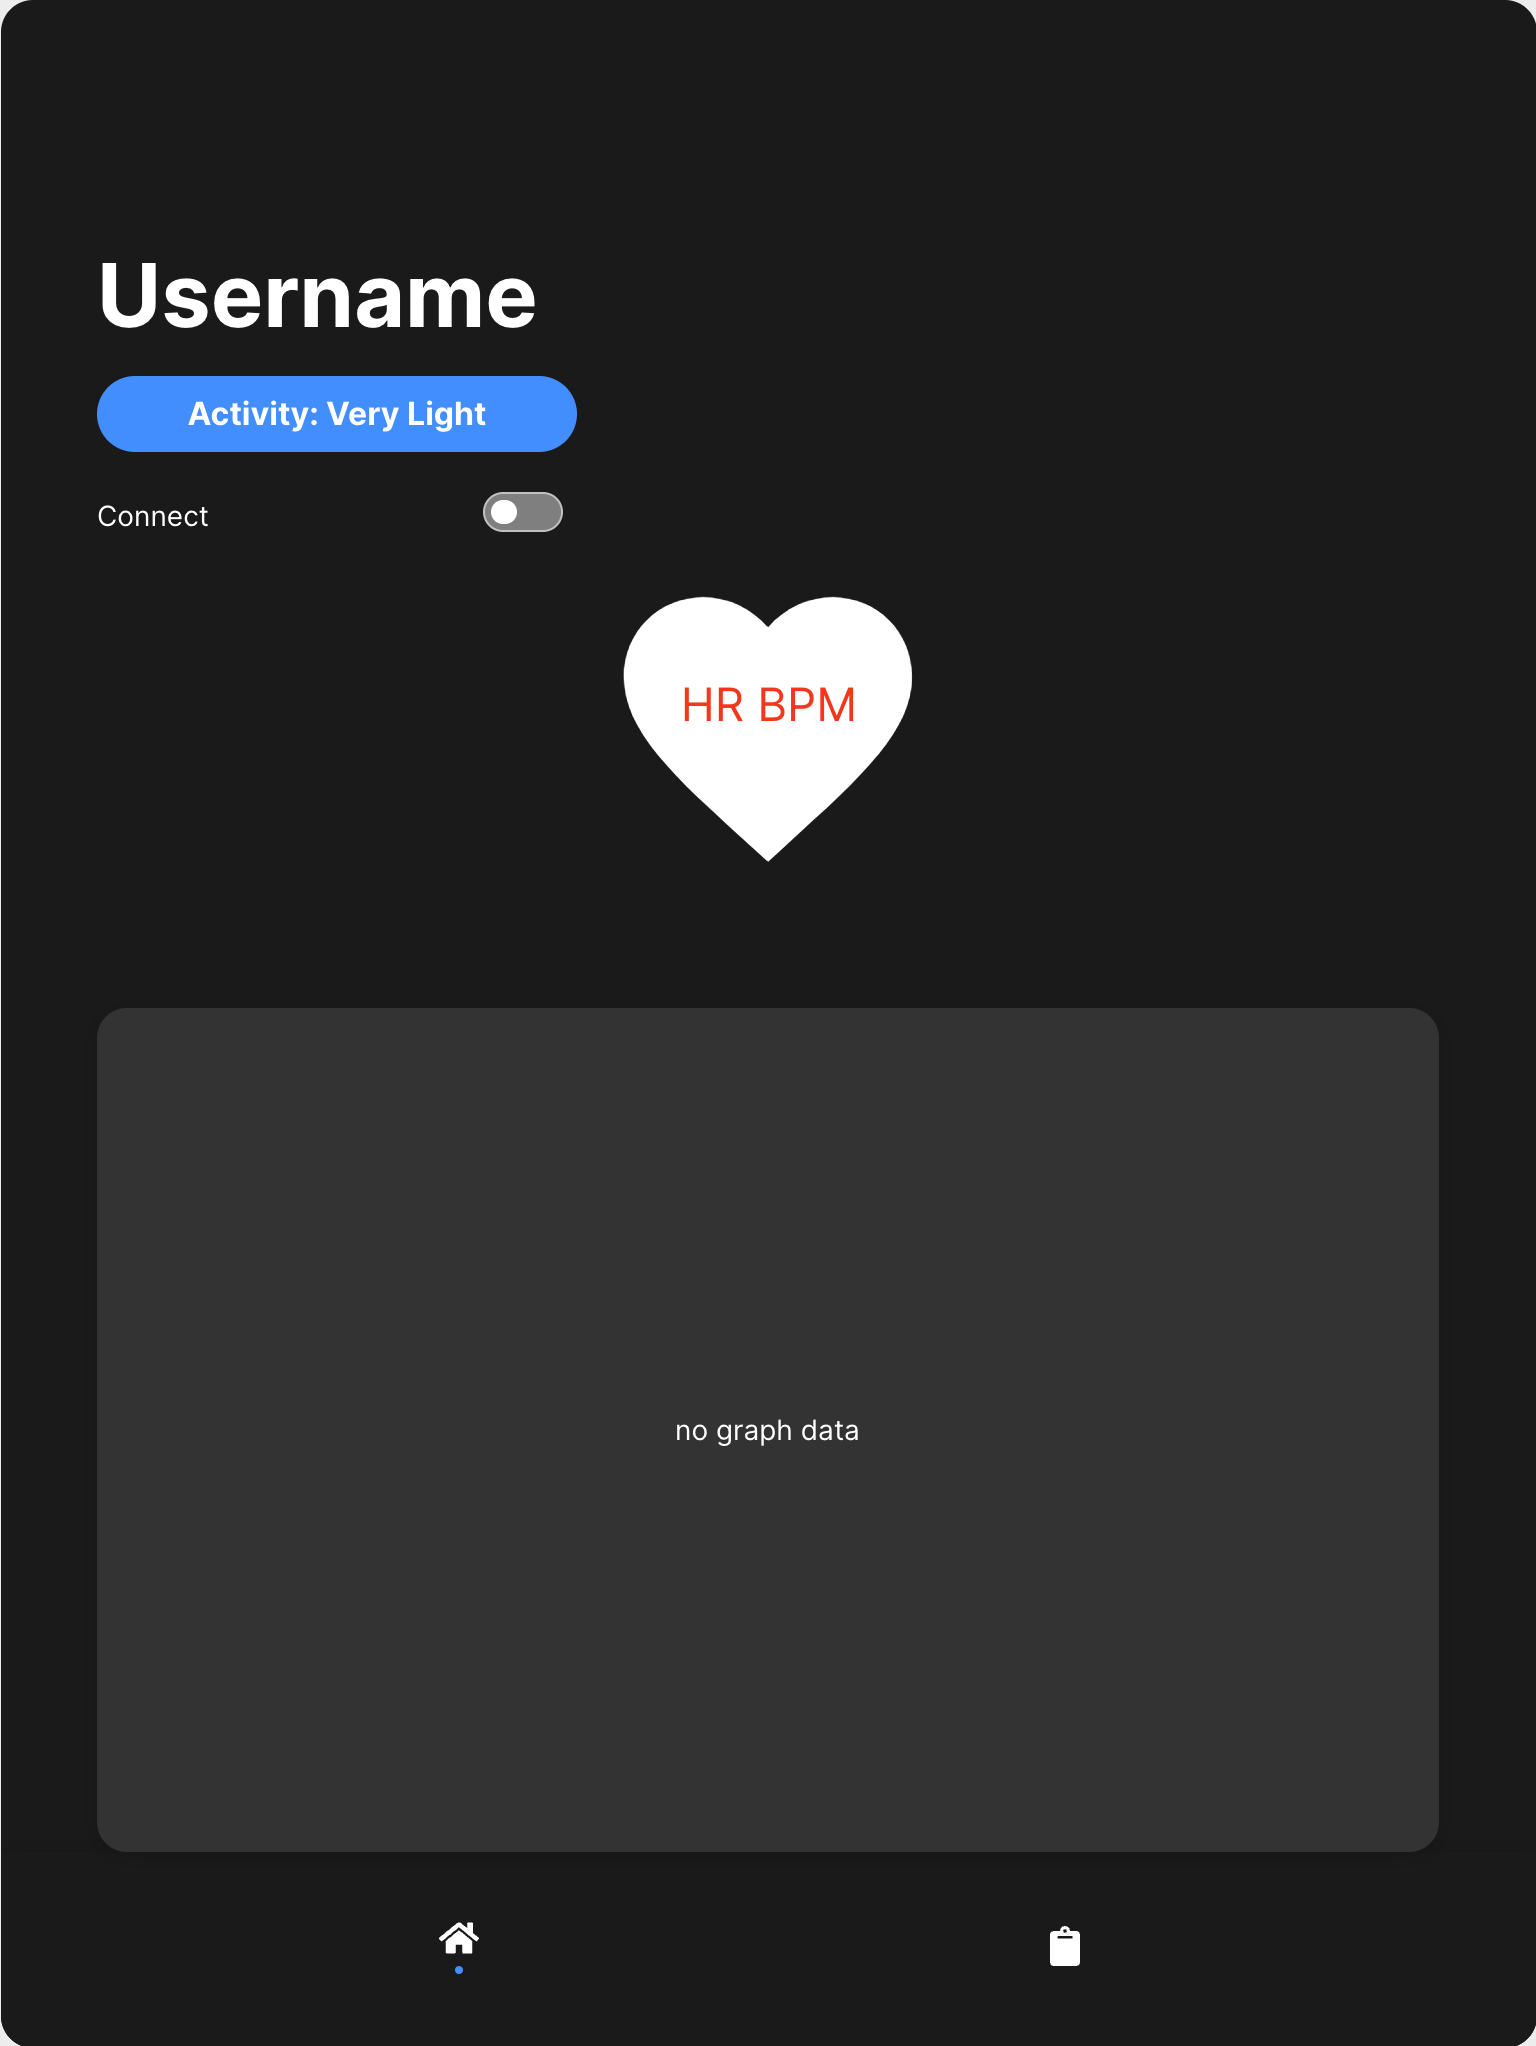
\includegraphics[width=0.75\textwidth]{images/home-fragment-mockup.png}
    \caption{HomeFragment mock-up}
    \label{fig:homefragment_mockup}
\end{figure}

